\chapter{IMPLEMENTATION}

\section{Core Controller Implementation}
The \texttt{ReportController} is responsible for handling report submissions, status updates, and dashboard logic. The following snippet shows how reports are stored with relevant department routing.

\begin{lstlisting}[style=phpstyle]
public function store(Request $request)
{
    $request->validate([
        'category' => 'required|string',
        'photo' => 'required|image|max:10240',
    ]);

    $photoPath = $request->file('photo')->store('reports', 'public');
    $map = Report::getCategoryDepartmentMap();
    $department = $map[$request->category] ?? null;

    Report::create([
        'user_id' => Auth::id(),
        'category' => $request->category,
        'department' => $department,
        'description' => $request->description,
        'photo_path' => $photoPath,
        'status' => 'Pending',
    ]);

    return redirect()->route('dashboard');
}
\end{lstlisting}

\section{User Interface Implementation}

\subsection{Landing Screen}
\begin{figure}[H]
    \centering
    
\includegraphics[width=0.9\textwidth]{images/landing_page.png}
    \caption{Implementation - Landing Page}
\end{figure}

\subsection{Dashboard Implementation}
\begin{figure}[H]
    \centering
    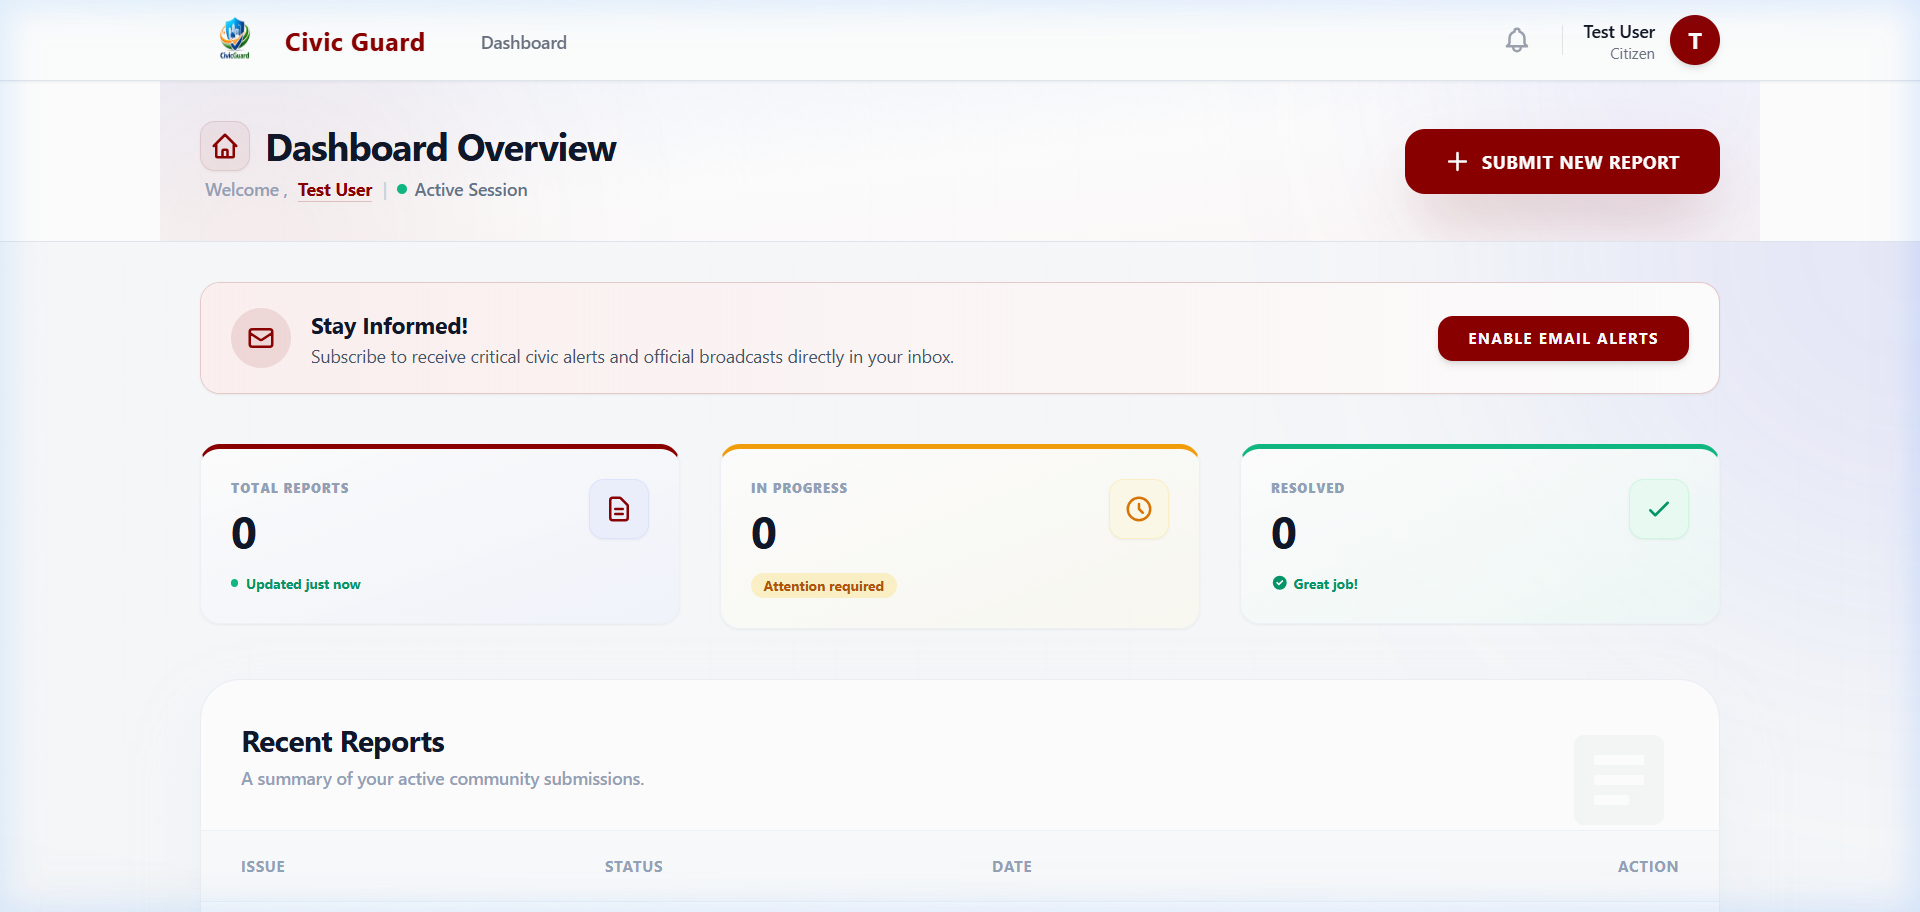
\includegraphics[width=0.9\textwidth]{images/dashboard.png}
    \caption{Implementation - Dashboard Overview}
\end{figure}

\subsection{Submission Form Implementation}
\begin{figure}[H]
    \centering
    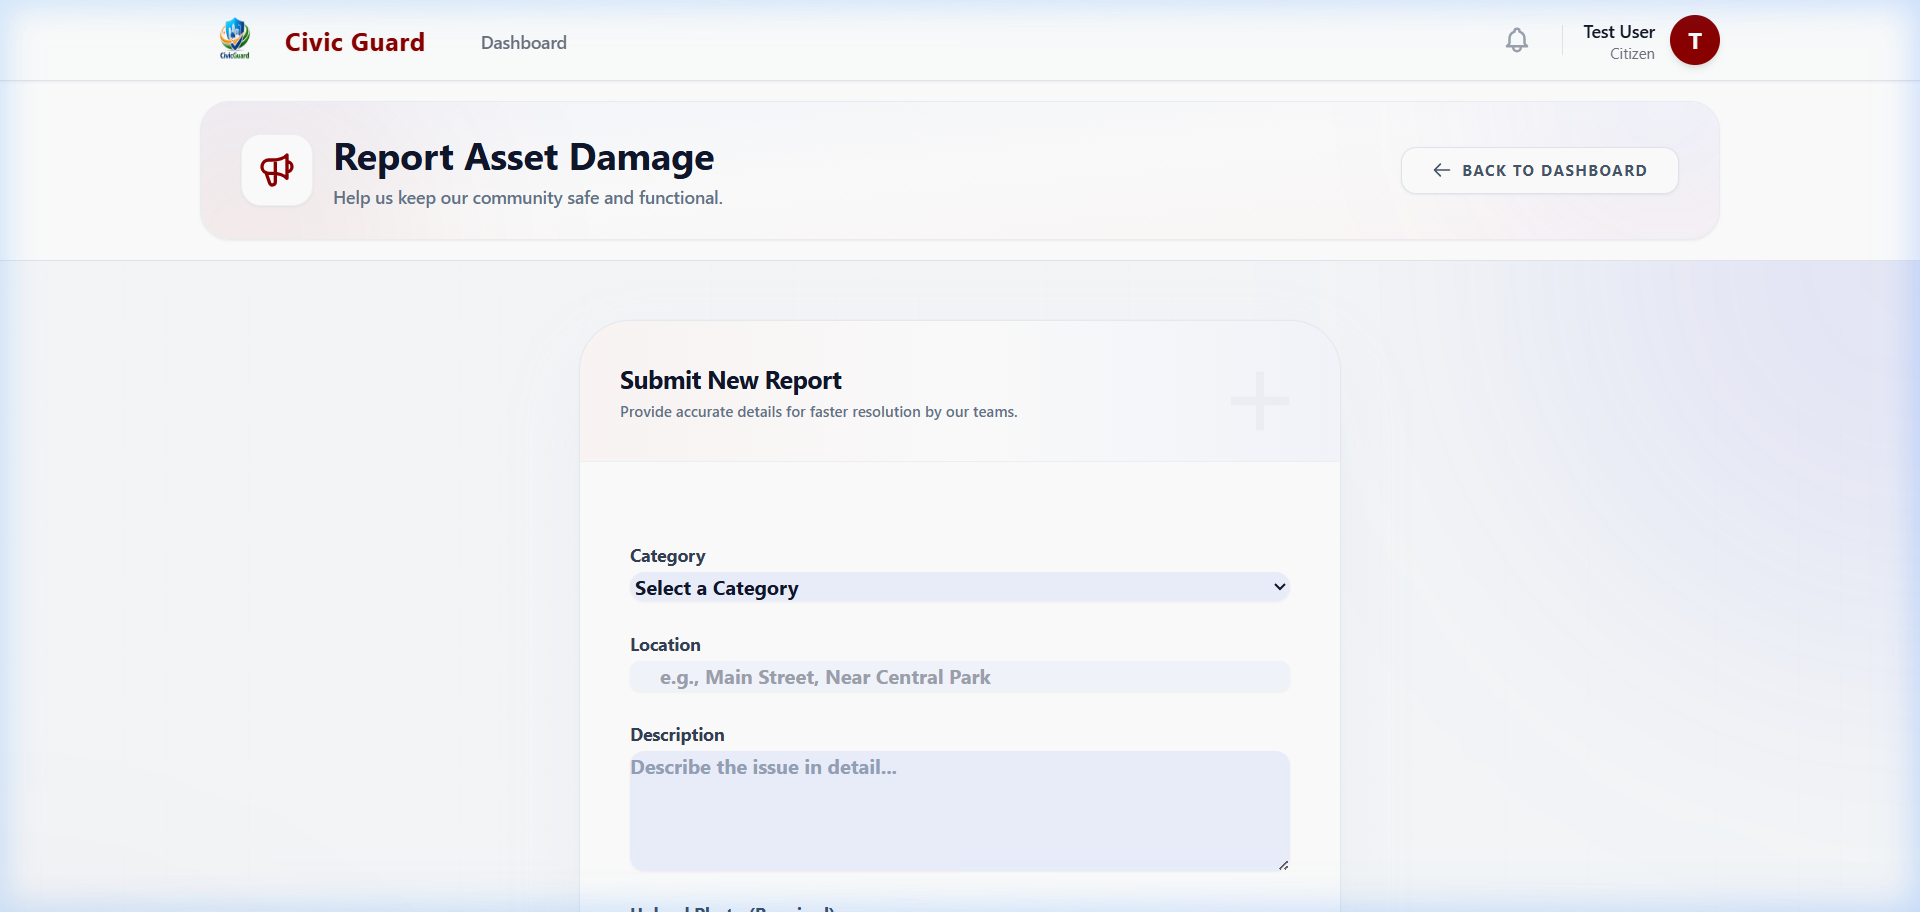
\includegraphics[width=0.9\textwidth]{images/report_creation.png}
    \caption{Implementation - Submission Form}
\end{figure}
The submission form uses Laravel's multipart form data handling to securely upload images and store them in the public storage disk, while recording the path in the database.
